\subsection{Récupération via scraping}
\vspace{1cm}

Pour avoir accès aux données indisponibles sous format Excel, il m’a fallut utiliser \colored{libcurl} pour récupérer le contenu du site actuel de la fédération.\\

Il s’agit d’une bibliothèque permettant de se connecter et de communiquer avec différents types de serveurs, et ce, avec différents types de protocoles. \\

Celle-ci m’a donc permis via le protocole HTTP de me connecter au site de la fédération avec des identifiants fournis par mon tuteur, de stocker les paramètres de connexion, et d’accéder au contenu HTML complet du site sous forme de chaîne de caractères.\\

Il m’a alors fallu analyser cette chaîne de caractères pour en tirer les informations qui m’intéressent, puis insérer celles-ci dans la base de données.

\subsubsection{Connexion}
\vspace{1cm}

Le langage PHP permet le support de \colored{libcurl} via l’extension `CURL` (Client URL Request Library), qui est disponible sous forme d’objet.

Celui-ci possède trois modules en fonction de l’utilisation voulue : un gestionnaire simple, un gestionnaire multiple et un gestionnaire de partage. Les ressources liées à ces gestionnaires sont respectivement \colored{CurlHandle}, \colored{CurlMultiHandle} et \colored{CurlShareHandle} depuis la version PHP8 \\

Dans le cadre de ma problématique, l’utilisation du gestionnaire simple était suffisante. Cependant, une connexion au site de la fédération était nécessaire avant toute récupération de contenu sur celui-ci. \\

Pour faire cela sans multiplier inutilement les connexion pour mes différentes requêtes, j’ai choisi de créer une classe permettant de configurer les paramètres de connexion et de les stocker dans l’objet \colored{CurlHandle} qui me permettait ensuite d’effectuer mes requêtes.

Une fois la connexion effectuée, un cookie était également généré par la librairie pour permettre l’authentification des prochaines requêtes.

\newpage

\begin{figure}[!h]
    \centering
    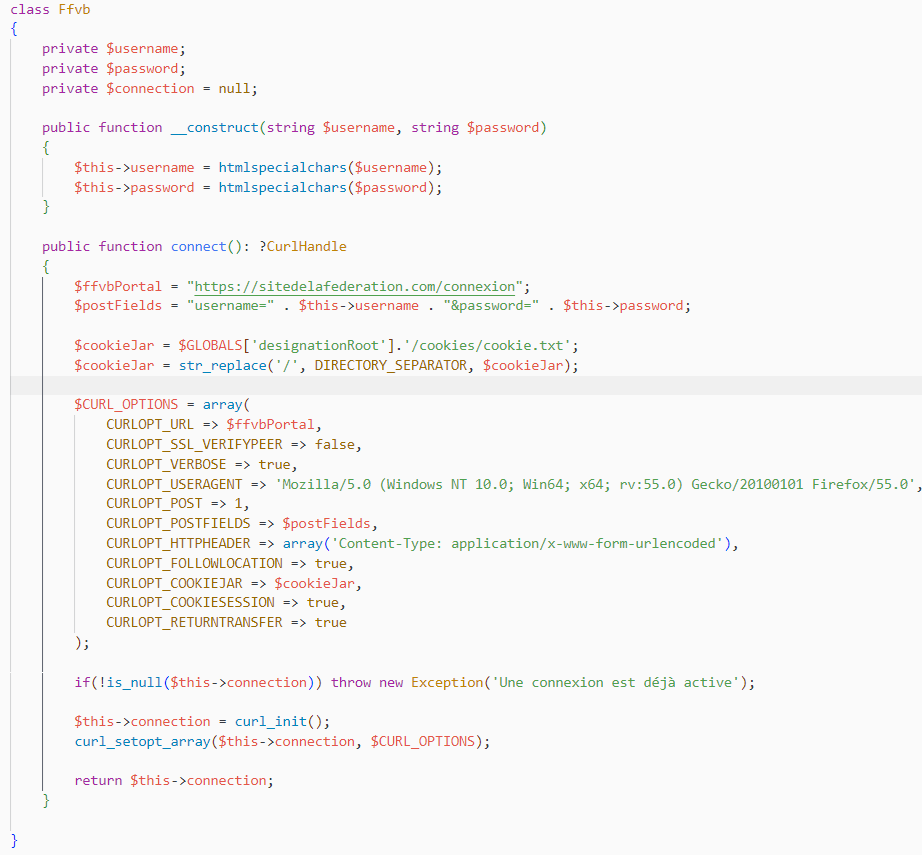
\includegraphics[width=\linewidth]{curl_code.png}
    \caption{Composant de paramétrage d'une connexion au site de la fédération}
\end{figure}

\newpage

\subsubsection{Analyse}
\vspace{1cm}

Les différents outils mis en place pour la récupération des données sur le site de la fédération prennent en paramètre le \colored{CurlHandle} de la connexion configuré précédemment pour effectuer leurs requêtes.\\

Après avoir défini le chemin vers les cookies de ma connexion, il m’a suffit d’envoyer une requête HTTP à la bonne URL pour y récupérer le contenu brut sous forme de chaîne de caractères.

\begin{figure}[!h]
    \centering
    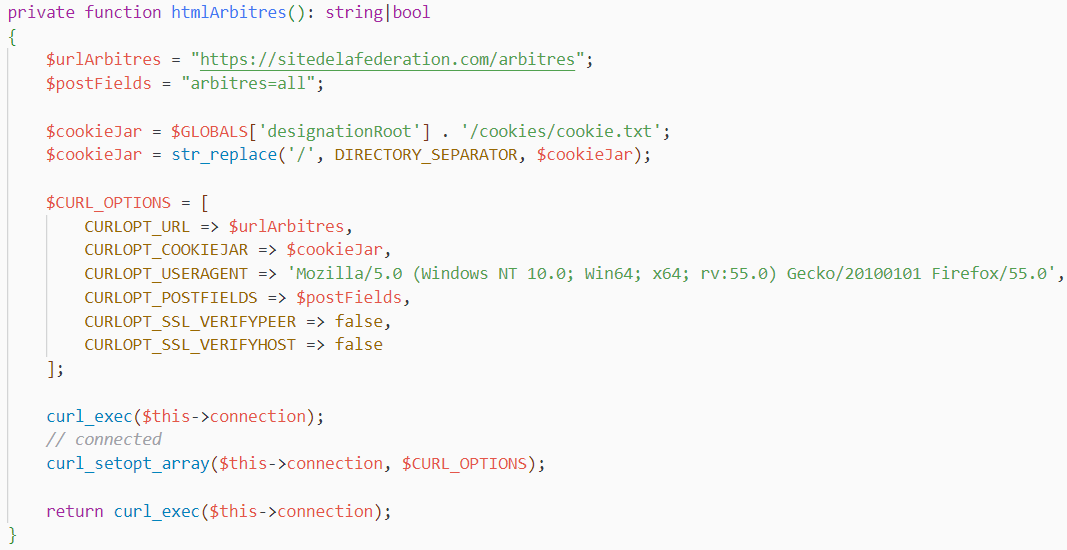
\includegraphics[width=\linewidth]{html_code.png}
    \caption{Méthode de récupération du contenu d'une page de l'intranet}
\end{figure}

\vspace{0.5cm}

Le contenu étant sous forme de chaîne de caractères, le principal problème était de récupérer seulement les informations utiles depuis cette String. Les données sont sous forme de tableaux, et le ciblage de ceux-ci est impossible dans cet état.

Heureusement, PHP possède nativement l’objet \colored{DOMDocument} qui permet d’analyser une chaîne de caractères afin de récupérer les éléments voulus comme nous l’aurions fait en JavaScript. 
En effet, cet objet possède plusieurs méthodes similaires et permettait donc de répondre à mon problème.\\

Cette étape d’analyse étant nécessaire pour toutes mes classes de récupération de données via \colored{CURL} , il m’a semblé logique de créer un objet spécialement conçu pour ça.

De plus, les données à récupérer étant pour la plupart sous forme de tableaux, j’ai également pensé à créer une méthode permettant de récupérer le détails des tableaux contenus dans une chaîne de caractères à partir de l’instance \colored{DOMDocument} liée à celle-ci.

\newpage

\begin{figure}[!h]
    \centering
    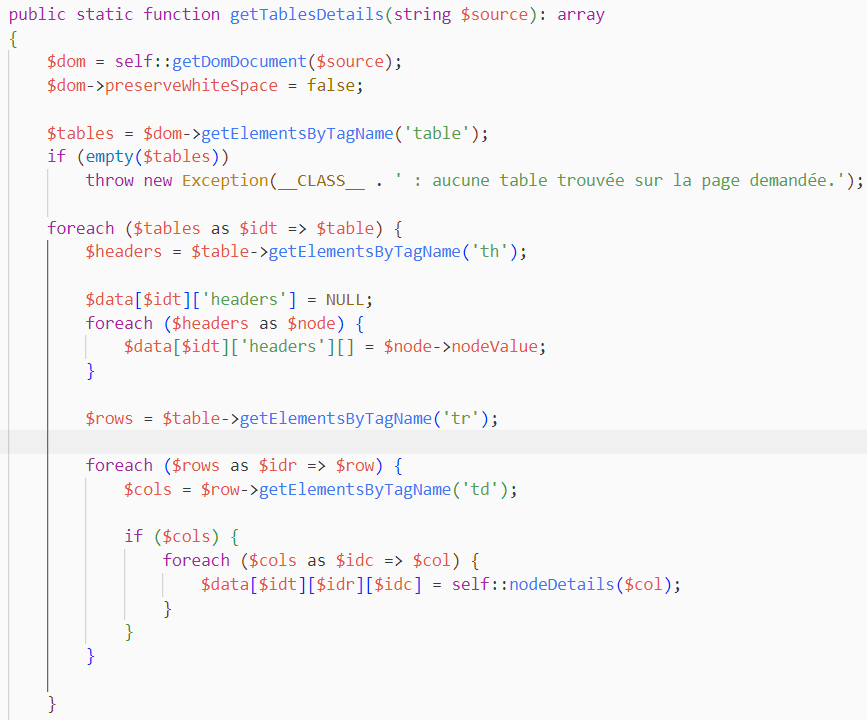
\includegraphics[width=\linewidth]{details_code.png}
    \caption{Méthode d'analyse du contenu d'une page HTML}
\end{figure}

\vspace{0.5cm}

Les détails des colonnes sont récupérés grâce à la méthode \colored{nodeDetails()} qui permet de scanner chaque colonne en récupérant le texte et les attributs si disponibles. Cette méthode effectue ce travail de façon dynamique pour chaque sous-nœud d’une colonne en se rappelant elle-même.

\newpage

\begin{figure}[!h]
    \centering
    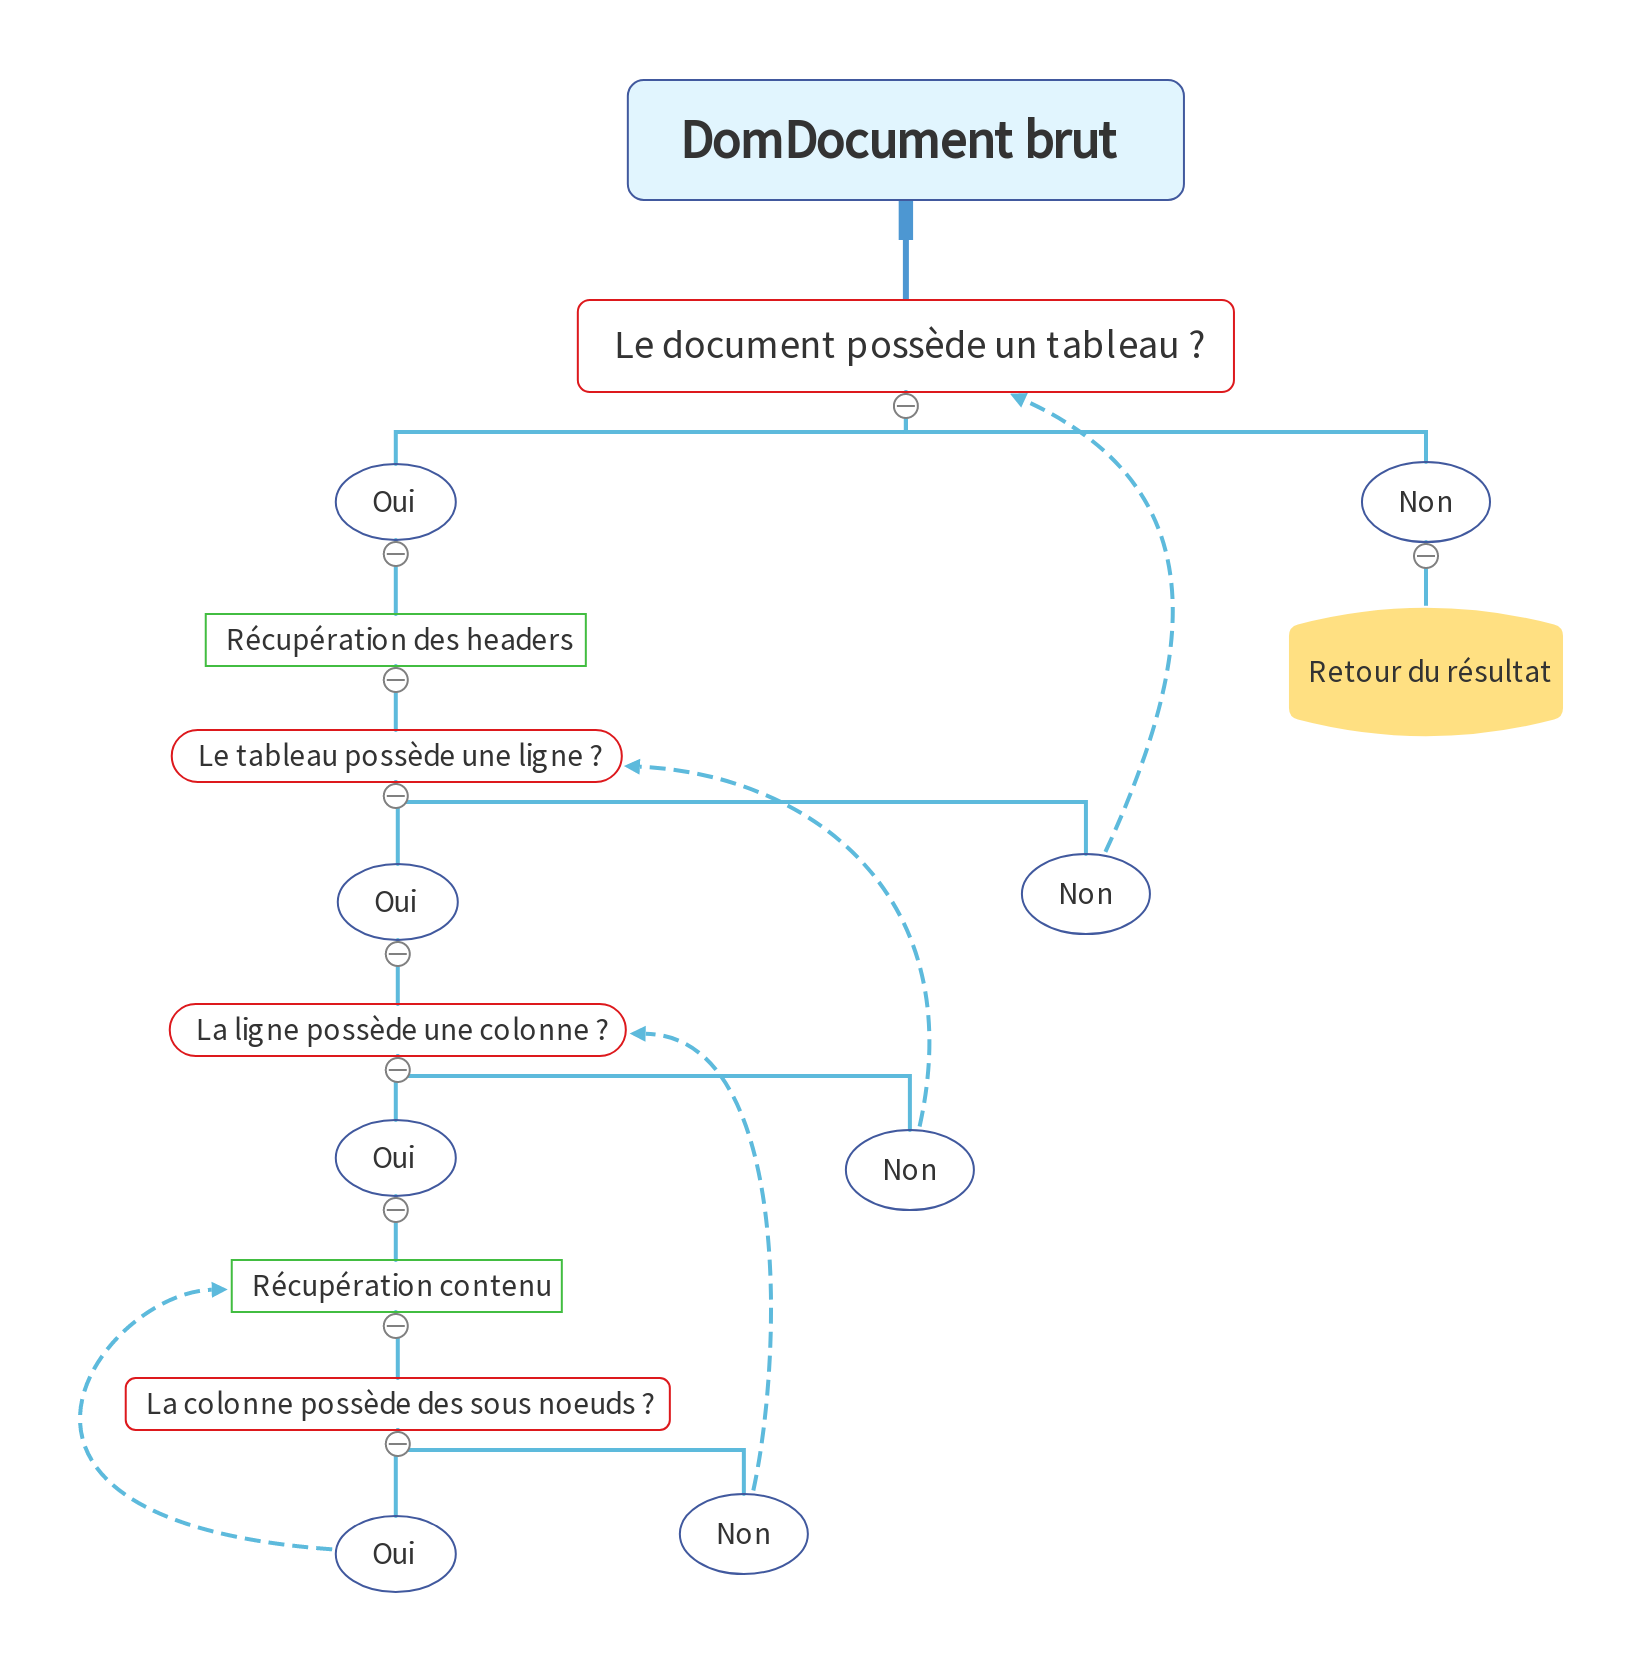
\includegraphics[width=\linewidth]{table_details.png}
    \caption{Logique suivie par la méthode d'analyse du contenu d'une page}
\end{figure}

\vspace{0.5cm}

Une fois ces objets et méthodes mis en place, la récupération et l’analyse des pages intéressantes du site de la fédération étaient beaucoup plus simples. 

J’ai donc ensuite créé une méthode propre à chacune de mes classes permettant de cibler et nettoyer les données renvoyées par les méthodes précédentes. Celles-ci ciblent les attributs et textes renvoyés par la méthode \colored{getTablesDetails()} pour afficher un tableau contenant l’essentiel des données voulues.

\newpage

\subsubsection{Insertion}
\vspace{1cm}

Pour stocker ces données dans la base de données, j’ai d’abord récupéré le nom des tables et colonnes concernées dans le fichier config.json (voir configuration), puis j’ai réutilisé ma classe Database pour effectuer une connexion avec celle-ci.

\begin{figure}[!h]
    \centering
    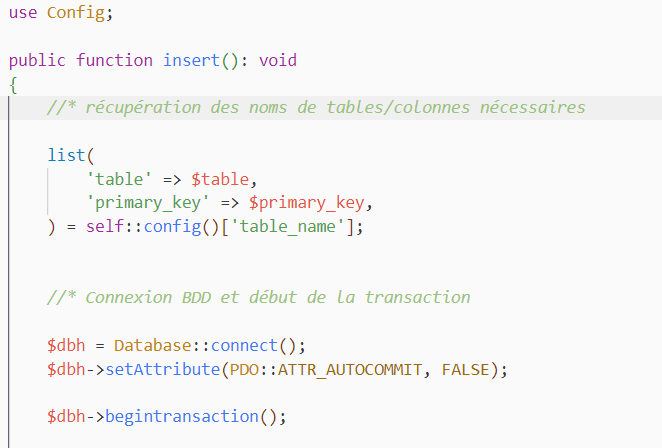
\includegraphics{insert1_code.png}
    \caption{Initialisation de l'insertion des données}
\end{figure}

Pour effectuer cette tâche de façon rapide et sécurisée, j’ai préféré utiliser des transactions et des requêtes préparées lors de la création des données. 
Les requêtes préparées permettent d’augmenter les performances en minimisant les allers-retours avec la base de données. 
Quant à elles, les transactions permettent d’éviter la perte de données dans le cas où certaines des requêtes ne passeraient pas.

De plus, l’objet PDO donne la possibilité de nettoyer les données lors de l’exécution en utilisant des variables nommées ou anonymes dans la requête, permettant ainsi d’éviter les \textbf{injections SQL}.

\begin{commentaire}
    Les injections SQL sont des méthodes permettant de détourner les requêtes SQL en injectant des bouts de codes malicieux.
\end{commentaire}

\begin{figure}[!h]
    \centering
    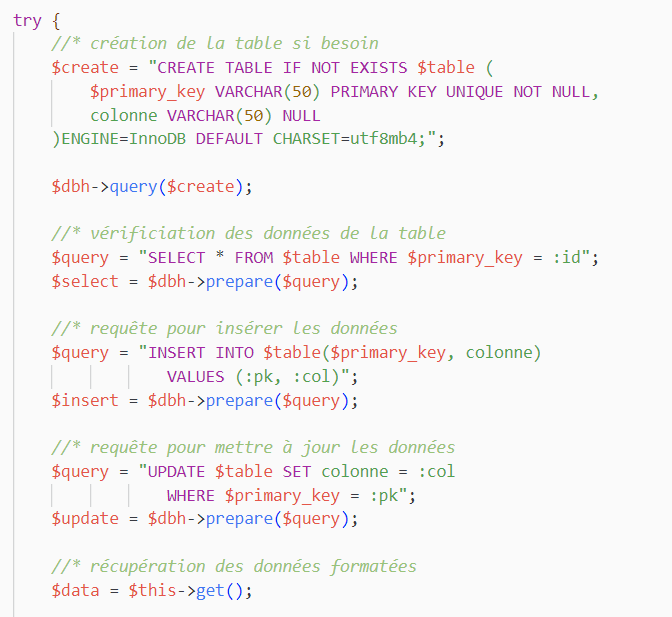
\includegraphics[width=12cm]{insert2_code.png}
    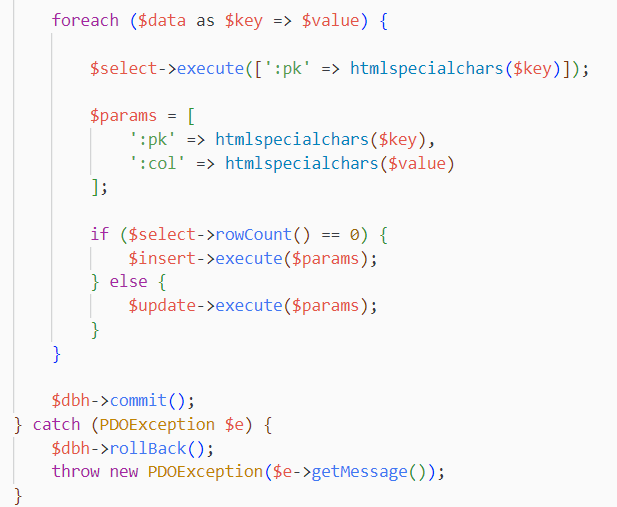
\includegraphics[width=12cm, height=10cm]{insert3_code.png}
    \caption{Insertion de toutes les données de façon sécurisée}
\end{figure}

\newpage

La logique de la méthode \colored{insert()} est de vérifier si les informations à insérer existent déjà dans la base de données, de les mettre à jour dans ce cas, et de les insérer dans le cas contraire. Ceci évite alors les erreurs SQL dues à la multiplicité des clés primaires.\\

Cette étape d’insertion des données m’a également permis d’uniformiser les données récupérées sur différents points d’entrées du site de la fédération, comme par exemples les matchs régionaux et nationaux.\\

En effet, les matchs régionaux et nationaux se trouvent sur deux parties différentes du site officiel et la récupération des informations liées à ceux-ci via scraping ne renvoient pas exactement le même type de données. Cette étape d’insertion était donc l’occasion d’uniformiser les informations qui seraient disponibles pour les uns mais pas les autres, en définissant des valeurs par défaut quand nécessaire.